\renewcommand{\thesection}{\Alph{section}}
To implement the system more effectively and efficiently, it is crucial to stabilize the development process. This provides a clear 
understanding of the tasks to be completed, their order of execution, and a reliable reference framework for teams working collaboratively 
on the same project. Therefore a proper planning for implementation and testing is essential. In following sections will be presented the
strategy in this phase of the project: the implementation plan, the integration plan, and the testing plan.

As the platform consists of several components and features, each with varying levels of complexity and dependencies on other components, 
the Bottom-Up is the suitable approach to optimize the development process. This approach allows team members to work independently on 
different parts of the system simultaneously. The process begins with the leaves of the "use" hierarchy and progresses upward toward the root.
This typically requires the creation of multiple drivers, one for each module. By following this approach, several subsystems will be developed 
and with the continuous integration of these subsystems, the final system will be created.

\section{Implementation Plan}\label{sec:implementation-plan}
The priority of components to be implemented is determined by their functionality and the dependencies between them. Since the system is divided 
into a set of components, as described in Section \ref{sect:architectural design}, the following list outlines the importance of each component
at the development stage, allowing for a smooth and efficient build process.
\begin{table}[H]
    \centering
    \begin{tabular}{|c|c|}
        \hline
        \textbf{Component} & \textbf{Priority} \\
        \hline
        Model Module & Very High \\
        \hline
        Notification Manager & Low \\
        \hline
        Authentication Manager & Medium \\
        \hline
        User Manager & High \\
        \hline
        Internship Manager & High \\
        \hline
        Application Manager & High \\
        \hline
        Recommendation Module & Medium \\
        \hline
        Search Module & Low \\
        \hline
    \end{tabular}
    \caption{Implementation Plan}\label{tab:implementation-plan}
\end{table}

 The Model Module serves as the foundation for all other components, meaning it is responsible for managing the platform's data. It facilitates
 communication between other components and the DBMS, providing an interface for accessing the data. Therefore, it should be implemented in 
 the first stage. Next, there is the Notification Manager supports communication between other components, such as the Authentication Manager, 
 Internship Manager, and Application Manager. After that, the Authentication Manager should be implemented, as it is an essential first step 
 for accessing the platform and controlling access to other components. Then following the dependency tree, the User Manager should then be 
 implemented which is responsible for managing user data and providing an interface for user-related operations. Once the basic components are
 are implemented, the core functions of the platform—the Internship Manager and Application Manager—can be developed. Afterward, the Search 
 Module and Recommendation Module can be implemented at the last stage, as they are secondary functions that are closely connected to the 
 platform's core functionalities.

\section{Integration Plan}\label{sec:integration-plan}
In this section will specify the order in which the components will be integrated and the components of each manager described in the
previous paragraph. The integration process will be divided into two main phases: the first phase will focus on integrating the components
of each manager, while the second phase will focus on integrating the managers themselves. Also during the integration process, the
unit testing and the integration testing will be performed to ensure that the components are working correctly by adding the functionalities
to the system.
\begin{enumerate}
    \item \textbf{Model Module:} The connection between the Model Module and the DBMS will be established first, as it is responsible for 
    managing the platform's data and providing an interface for other components to access the data.
    \begin{figure}[H]
        \centering
        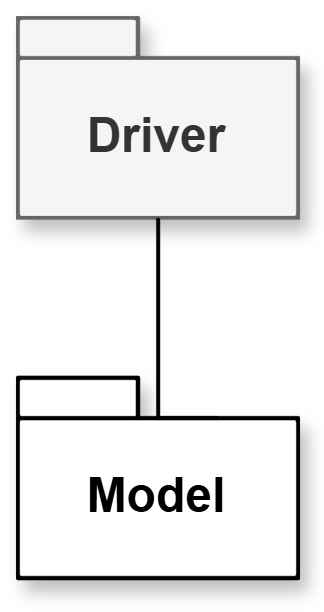
\includegraphics[width=0.16\textwidth]{Images/BottomUp/Model.png}
    \end{figure}
    \item \textbf{Notification Manager:} The Notification Manager will be integrated next with the Model Module, at this stage, the connection
    between the Notification Manager and the Model Module will be established and tested.
    \begin{figure}[H]
        \centering
        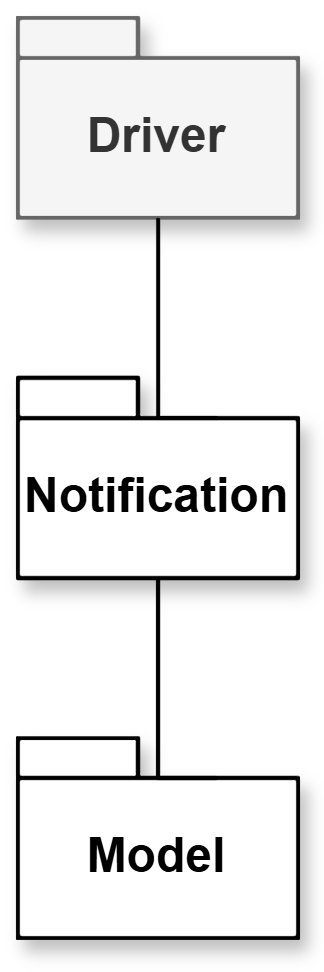
\includegraphics[width=0.2\textwidth]{Images/BottomUp/Notification.png}
    \end{figure}
    \item \textbf{Authentication Manager:} The Authentication Manager, including the Registration and Login Manager, will be integrated next, 
    as these are the basic functionalities for accessing the platform. After interaction with the Model Module and the Notification Manager, 
    their functionalities will be tested to ensure that reading and writing operations in the database work correctly and that notifications 
    are sent properly during the registration and login processes. Additionally, the communication with the external email service will be verified.
    \begin{figure}[H]
        \centering
        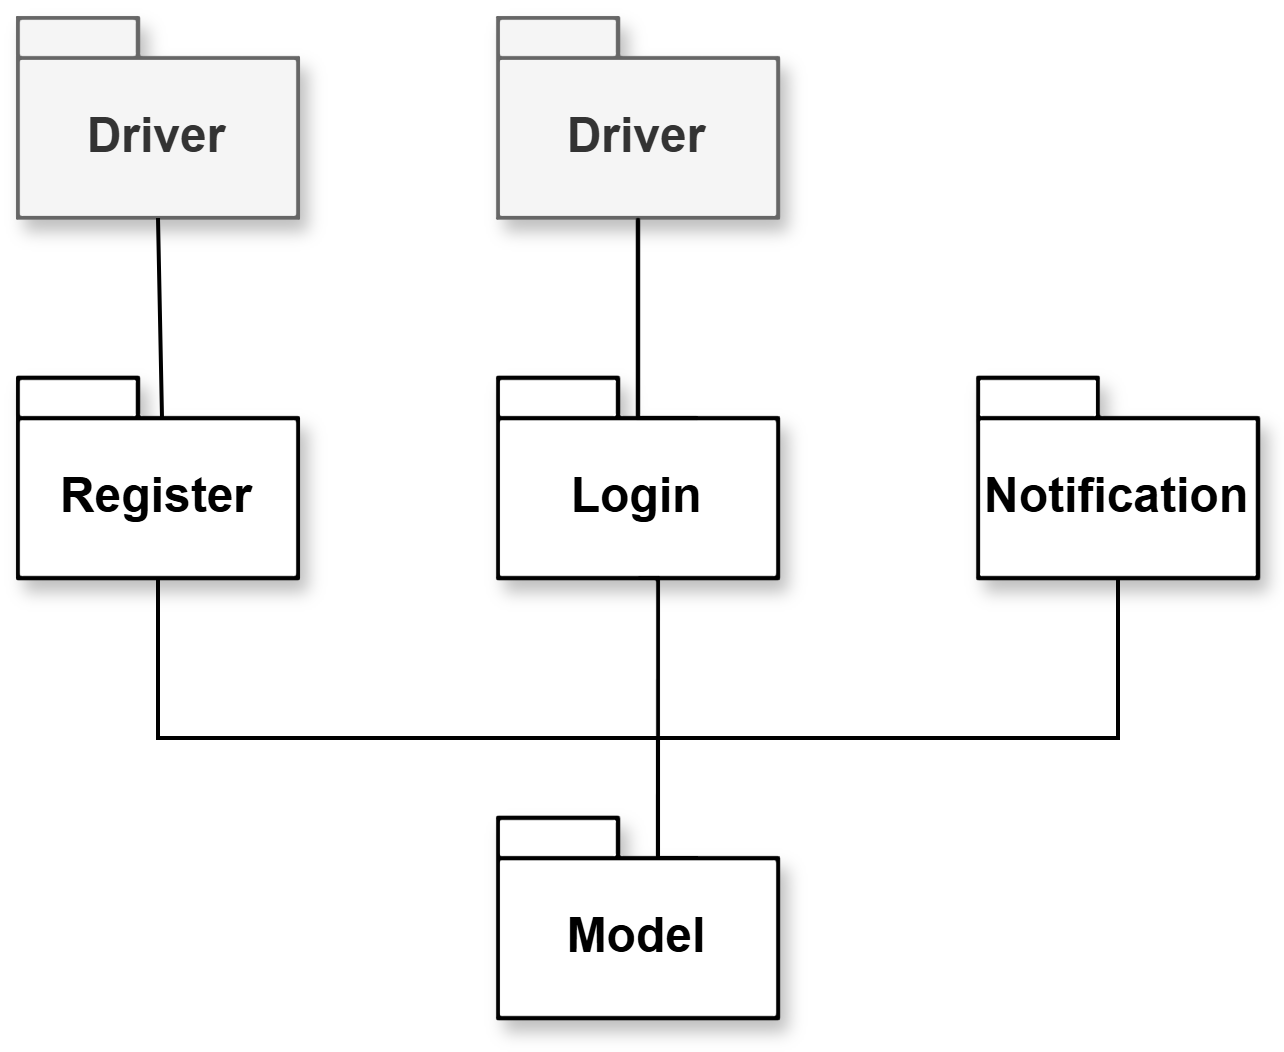
\includegraphics[width=0.4\textwidth]{Images/BottomUp/Auth.png}
    \end{figure} 
    \item \textbf{User Manager:} As the last basic component, the View Profile Manager and Profile Modification Manager will be integrated. 
    Since they depend only on components that have already been integrated, unit testing and integration testing can be conducted to ensure that 
    all basic functionalities work correctly before moving to the integration of the core functionalities.
    \begin{figure}[H]
        \centering
        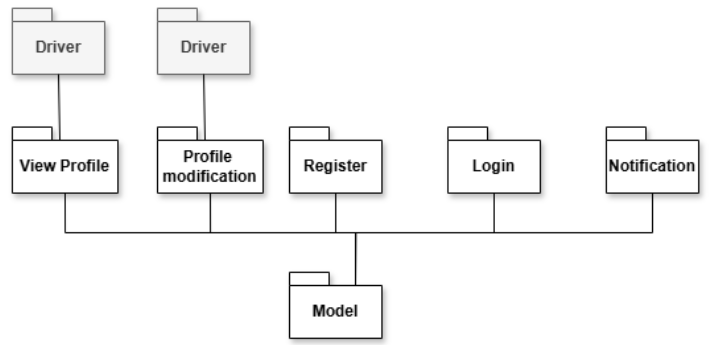
\includegraphics[width=0.7\textwidth]{Images/BottomUp/Profile.png}
    \end{figure}
    \item \textbf{Internship Manager:} The Internship Manager is the first core functionality to be integrated, as it is responsible for managing 
    internship data and providing an interface for internship-related operations. The order of integration of its components is as follows: 
    Creation Manager, View Internship Information Manager, Selection Manager, Chat Manager, and Feedback Manager, reflecting the order of processing 
    internship evolution. Unit testing is crucial at this stage, and extreme cases should be evaluated. Mock data will be used to simulate real 
    internship events. Integration testing of all components integrated so far will also be conducted to ensure that everything works without 
    conflicts or crashes.
    \begin{figure}[H]
        \centering
        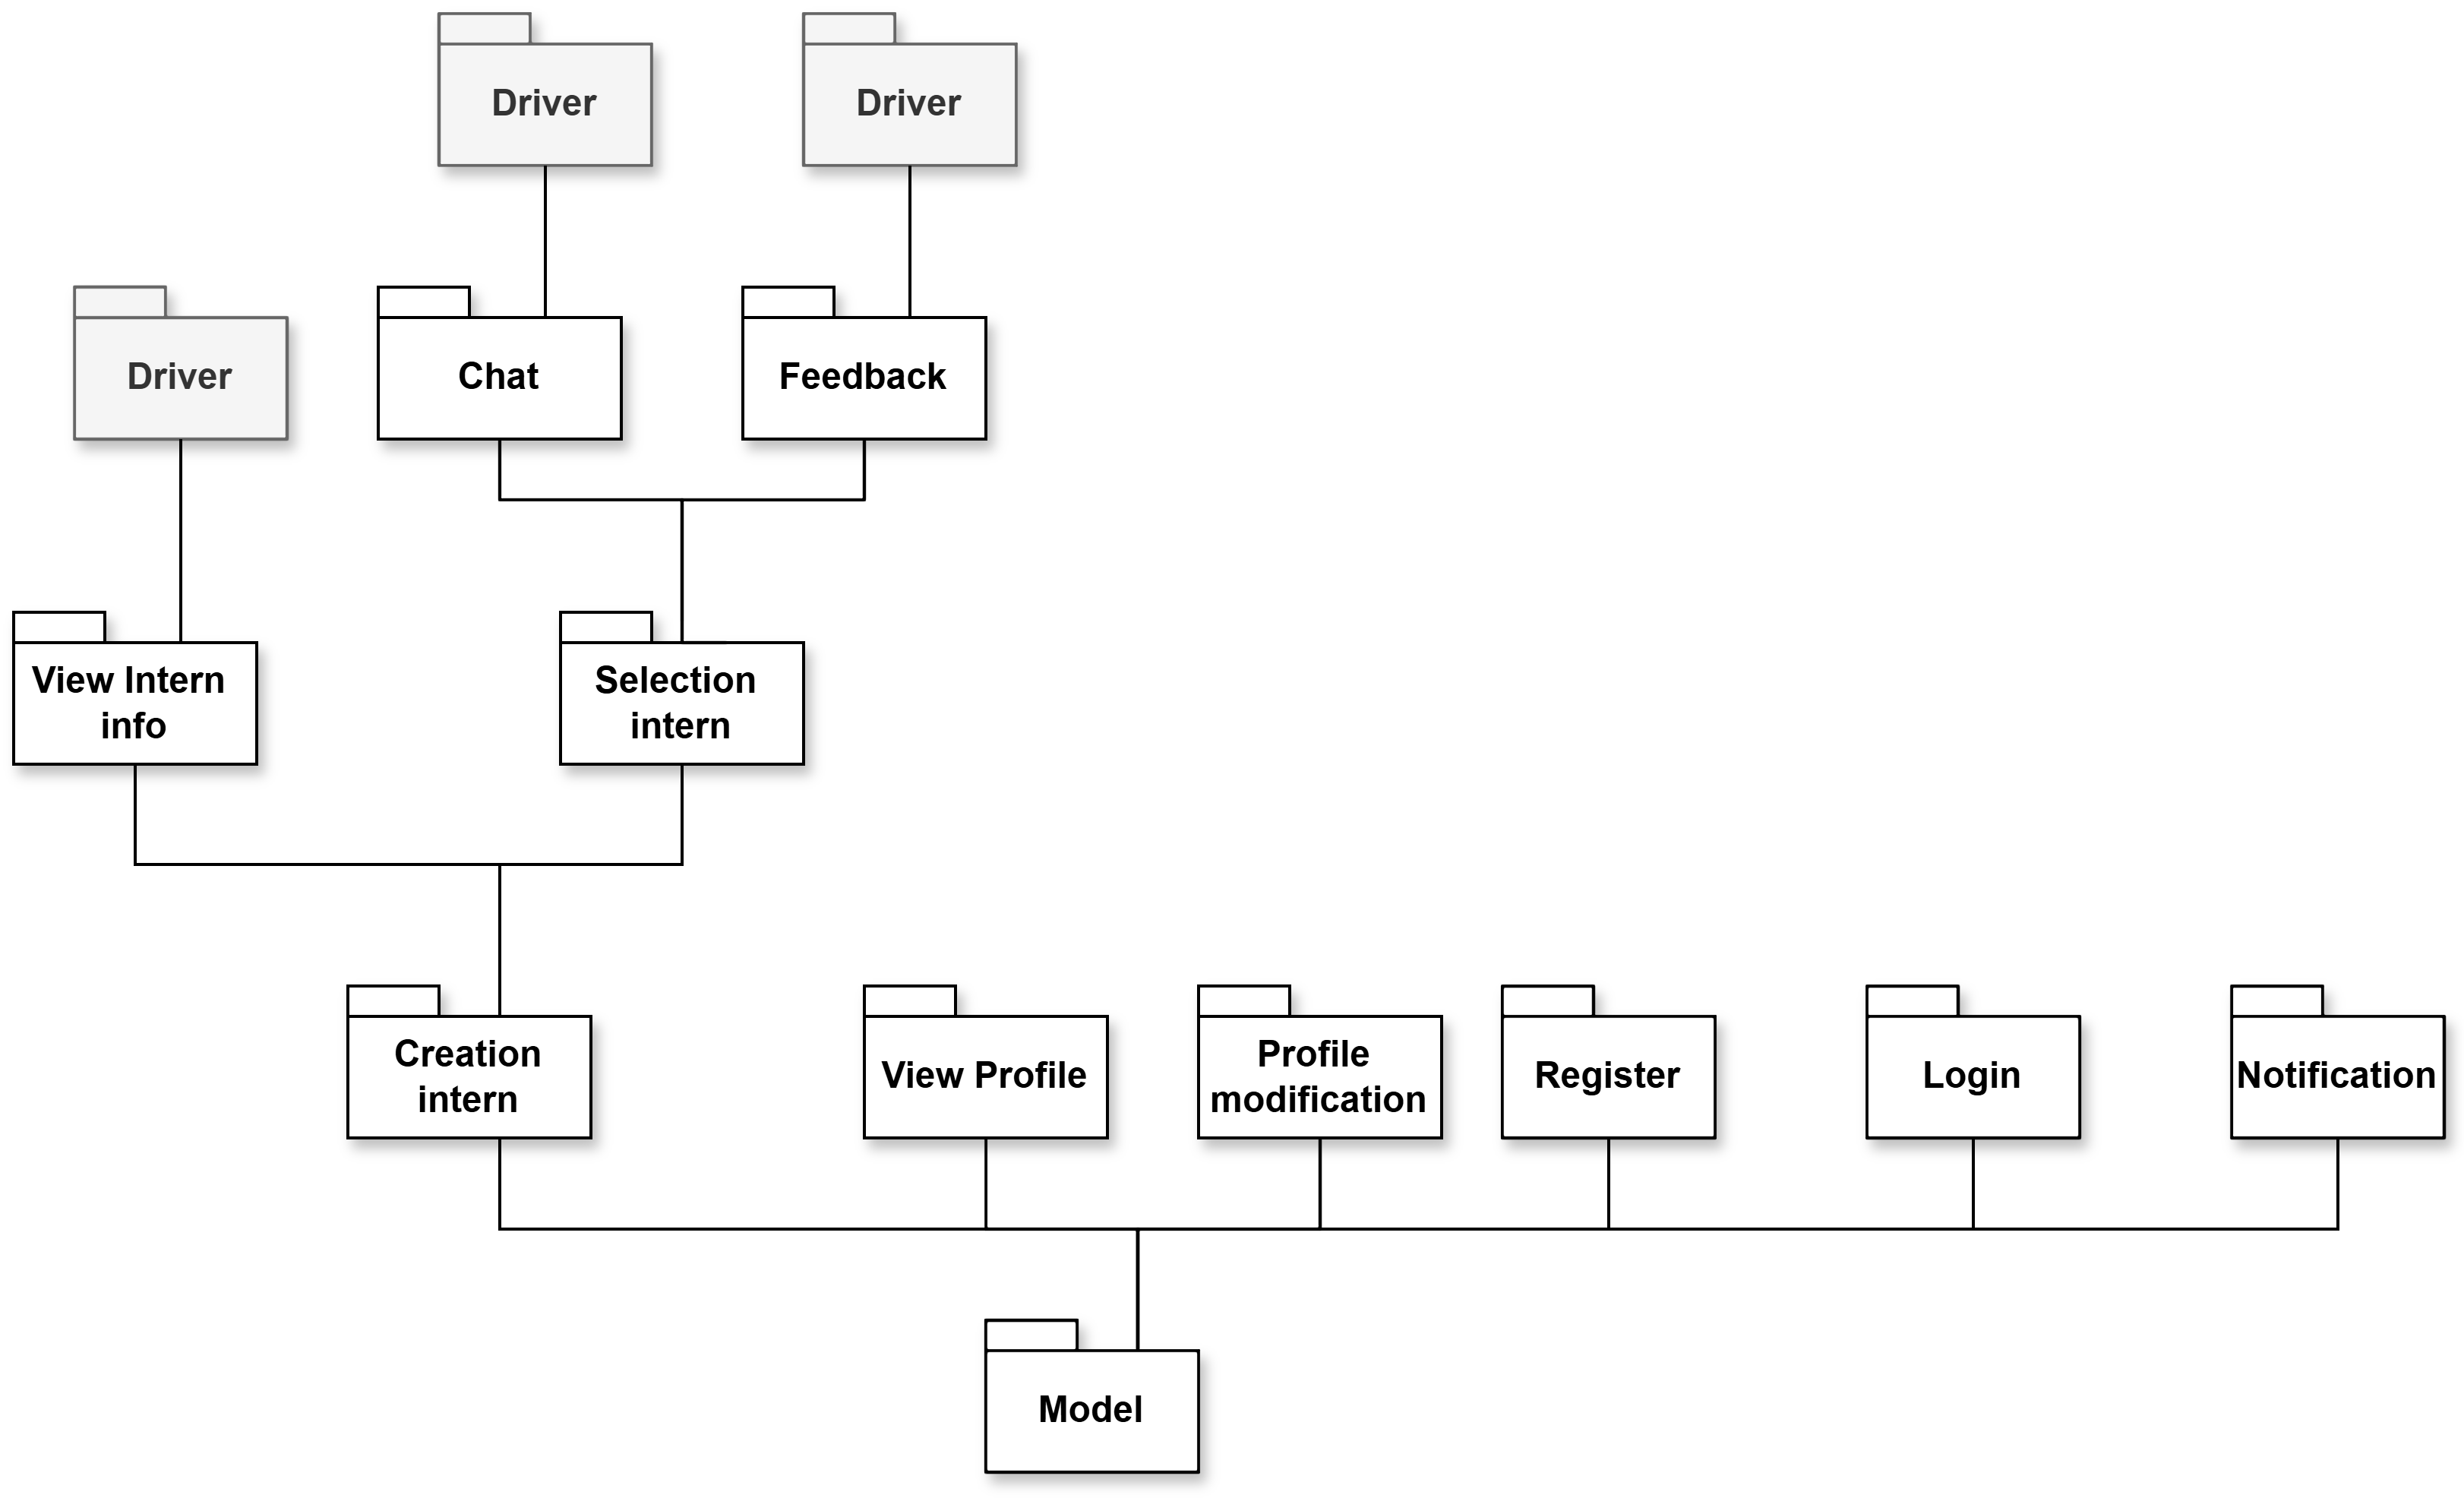
\includegraphics[width=1\textwidth]{Images/BottomUp/Intern.png}
    \end{figure}
    \item \textbf{Application Manager:} Next, the Application Manager, which manages applications and controls the selection process, will be integrated. 
    The order of integration of its components is as follows: Submissions Manager, View Application Information Manager, Interview Manager, and 
    Questionnaire Manager. It must collaborate seamlessly with the Internship Manager and the User Manager. Integration testing is critical during 
    this phase since the platform's main functionalities are involved.
    \begin{figure}[H]
        \centering
        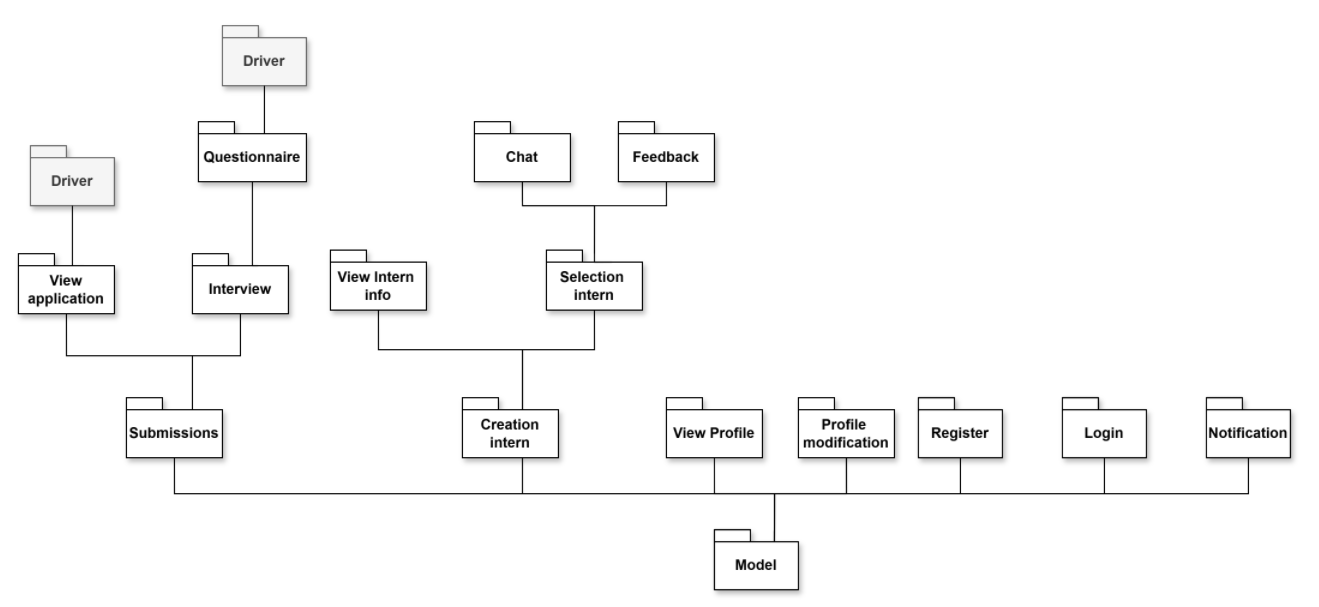
\includegraphics[width=1\textwidth]{Images/BottomUp/Application.png}
    \end{figure}
    \item \textbf{Recommendation Module:} After integrating and testing the core and basic functionalities, the Recommendation Module will be integrated. 
    This module depends on all previously developed components. Testing of the recommendation algorithm will be performed to verify that it provides 
    suitable recommendations based on the user's profile and internship experiences. 
    \begin{figure}[H]
        \centering
        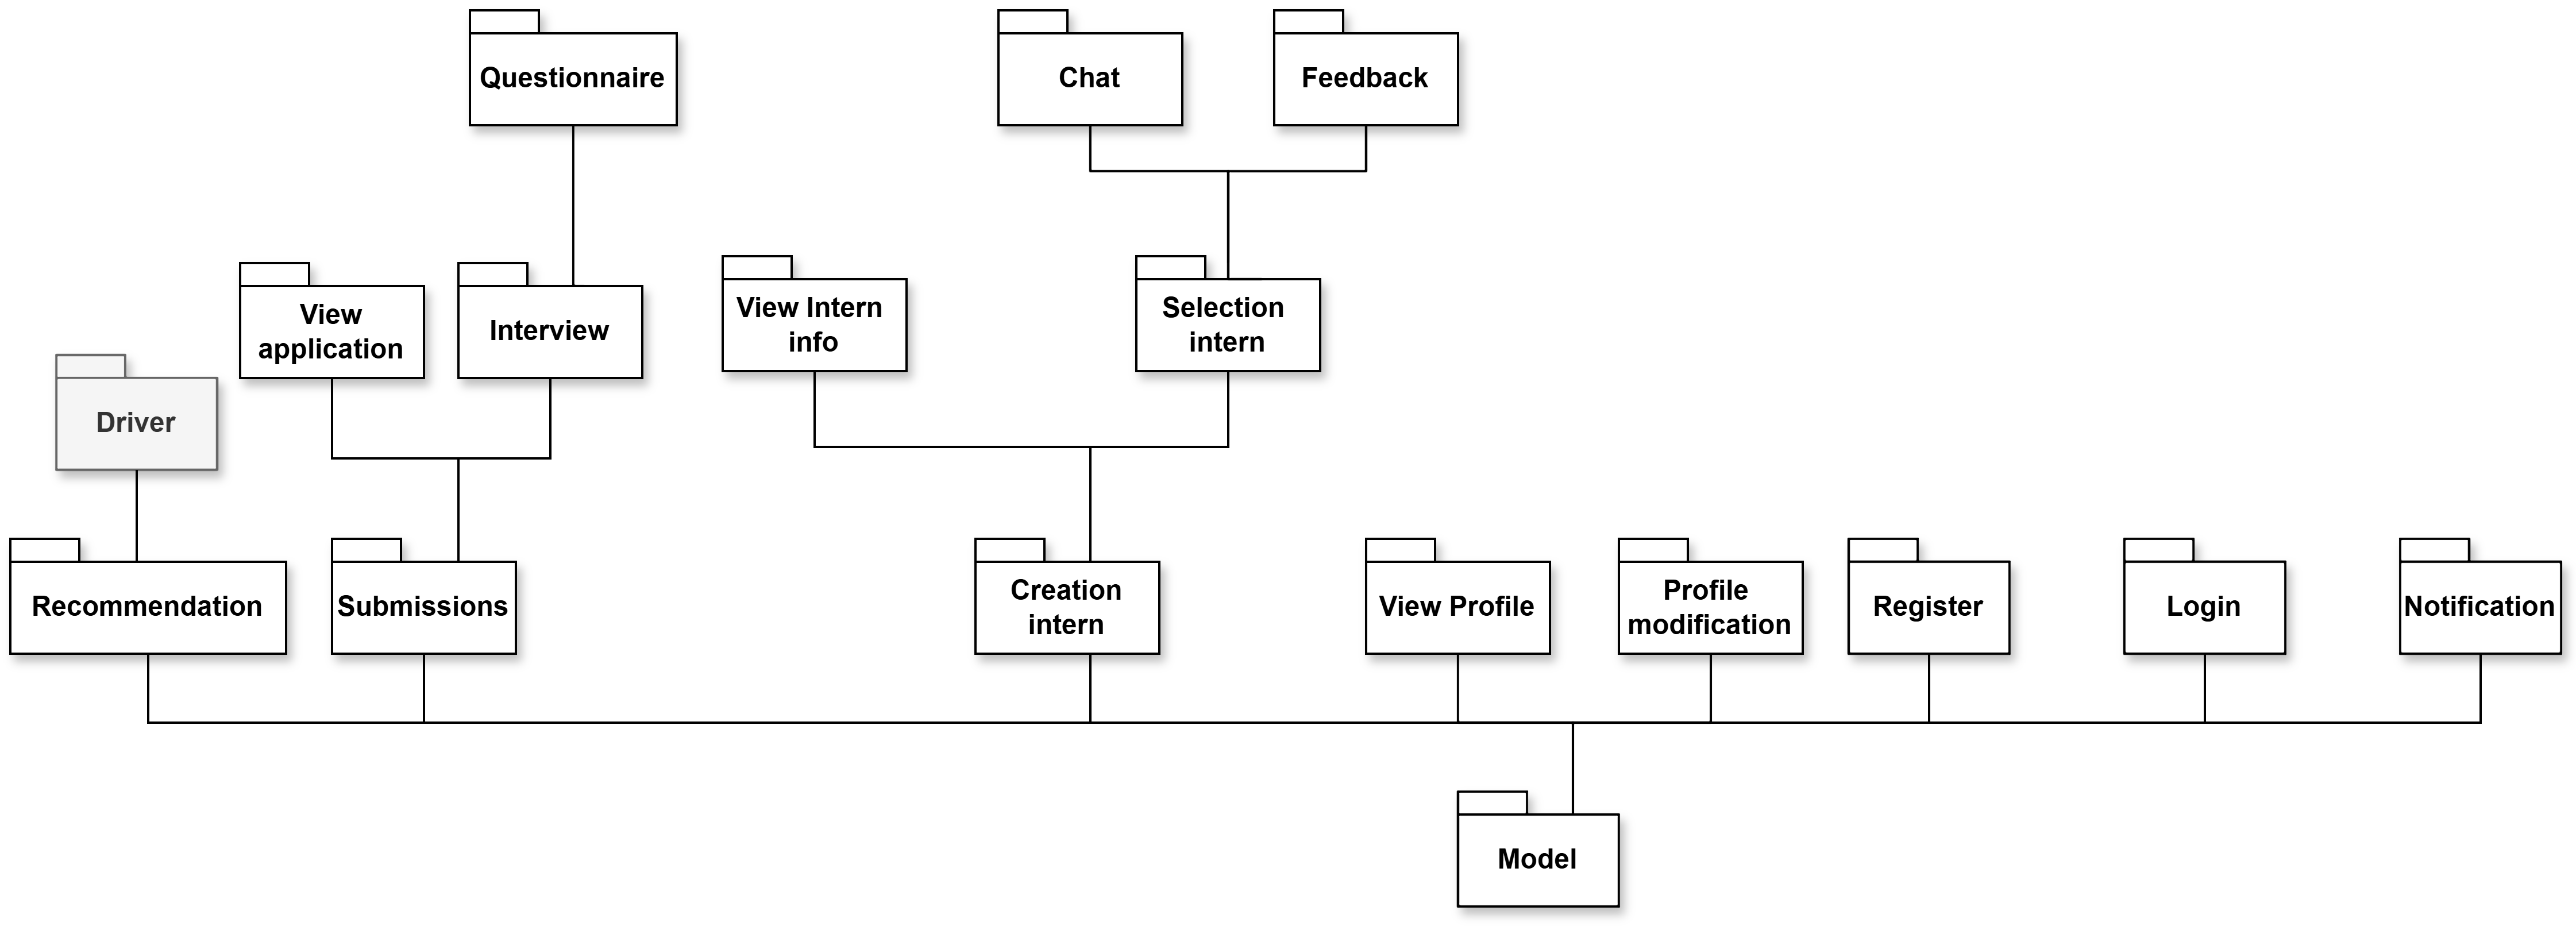
\includegraphics[width=1\textwidth]{Images/BottomUp/Recomm.png}
    \end{figure}
    \item \textbf{Search Module:} Even though the Search Module is not closely related to all components developed so far, it will be integrated at the
     end of the integration process. This is because it is a secondary function closely connected to the platform's core functionalities. Once all other
      components have been integrated and tested, the Search Module can be integrated and tested. This approach ensures that any issues with the search 
      functionalities are not caused by other components.
      \begin{figure}[H]
        \centering
        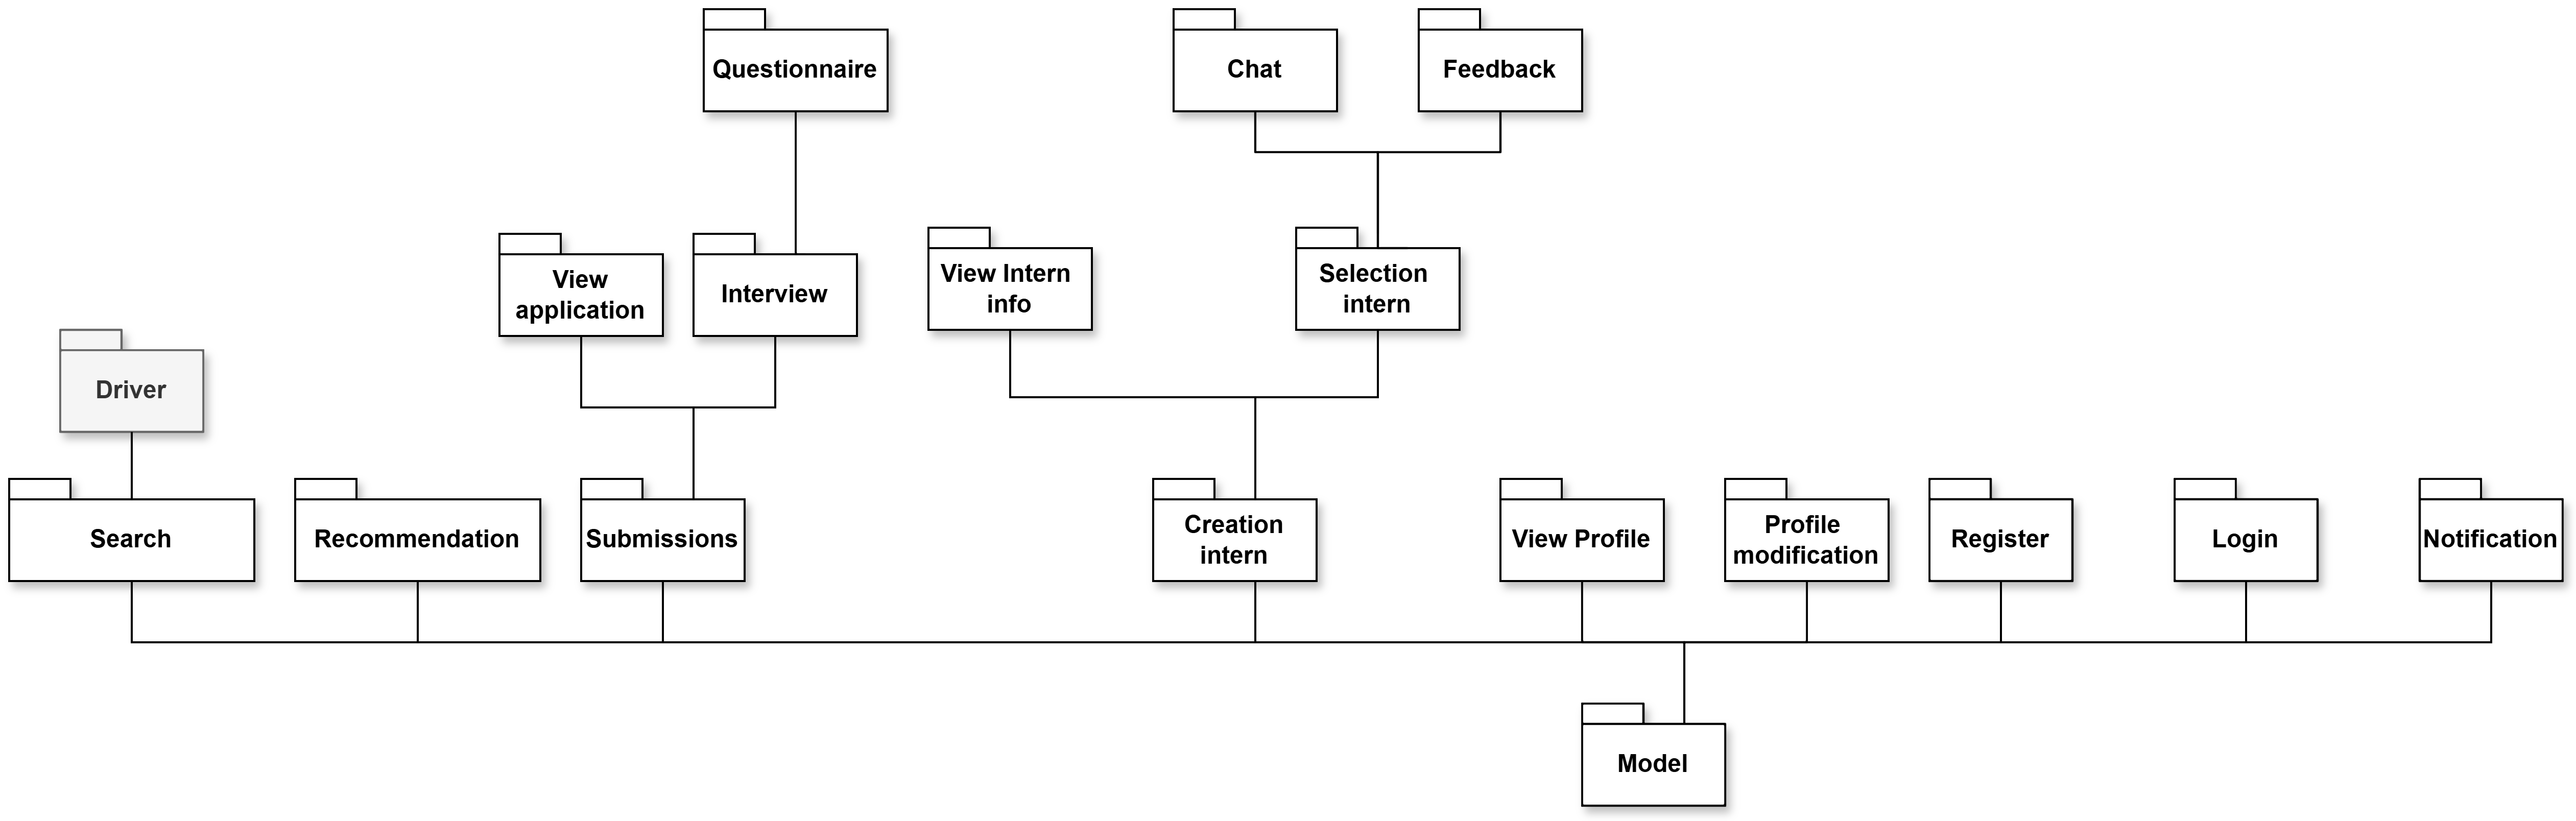
\includegraphics[width=1\textwidth]{Images/BottomUp/Search.png}
    \end{figure}
    \item After completing the server-side integration, the client-side integration will be performed. The integration of server-side components with 
    client-side components will be processed, and testing of the interaction between server-side and client-side components will be conducted.
\end{enumerate}

\section{System Testing}\label{sec:testing-plan}
After the iterative testing process during the integration of the components, once the system is fully integrated, it needs to be tested as a whole
 using other testing techniques. In this section, the testing will focus on identifying any issues with the system's functionalities and determining 
 whether all the requirements are satisfied. During this phase, all different roles of project members will be involved in the testing process, 
 including developers, users, and black-box testers.
    \begin{itemize}
        \item \textbf{Functional Testing:} Functional testing is used to check if all functional requirements indicated in the RASD are fulfilled by 
        the software. Communication between different stakeholders and users is important to understand if the functionalities are truly as expected. 
        \item \textbf{Load Testing:} Load testing will check if the platform can handle the expected load, and if there are any bugs, such as memory 
        leaks, mismanagement of memory, or buffer overflows. It will also identify the upper limits of the components and help evaluate the optimal 
        architectural options. The system will be tested with increasing workloads until it reaches its capacity.
        \item \textbf{Performance Testing:} Performance testing aims to detect bottlenecks, inefficient algorithms, hardware or network issues, and
         to identify more efficient solutions to achieve specific goals. It should take into consideration response time, utilization, and 
         throughput of the system.
        \item \textbf{Stress testing:} Stress testing ensures high maintainability and availability. It verifies that the system recovers gracefully 
        after unexpected failures or crashes. The system should be tested by overwhelming its resources or reducing resources, for example, by 
        randomly shutting down and restarting ports on a network switch to observe the system's behavior.
        \item \textbf{User Interface Testing:} User interface testing is essential to ensure that the connection between the client and the server
        is established smoothly. It will also verify that the user interface is user-friendly and that the user can easily navigate from the user's
        perspective.
    \end{itemize}


